\chapter{Boundary layer climatology of New York City}
\label{chapter:climatology}
\thispagestyle{myheadings}

% set this to the location of the figures for this chapter. it may
% also want to be ../Figures/2_Body/ or something. make sure that
% it has a trailing directory separator (i.e., '/')!
\graphicspath{{3_Pub2/}}

%%%%%% Packages
% Handles references

%%%%% Introduction
\section{Introduction} \label{section:introduction}

Extreme heat poses a major risk to life and property. The effects of extreme heat are expected to impact cities especially, presenting a significant hazard for vulnerable populations and infrastructure. With regards to effects on public health, studies have shown that extreme and prolonged heat increases mortality and exacerbates existing health conditions in high-risk populations \citep{anderson2011, frumkin2016, heaviside2017, madrigano2015}. With regards to effects on infrastructure, studies have shown that extreme heat subjects networks critical to urban areas (e.g., electrical grid, public transportation) under significant stresses and/or failure \citep{mcevoy2012, zuo2015}. These events are projected to increase in frequency due to the effects of climate change. Projections indicate that the impacts of future climate will cause adverse effects of extreme heat on cities to become more frequent and severe \citep{burillo2019, forzieri2018, peng2011}.

% Comment: try to couple the local and the mesoscale here
The meteorology of extreme heat events and its impacts on urban areas can be observed from the synoptic and local scales. From a synoptic scale, extreme heat events are often caused by the sustained presence of a high-pressure system over an area, resulting in lower horizontal wind speeds and warm air subsidence, promoting higher surface temperatures \citep{black2004, miralles2014}. From a local perspective, the amplified impact of extreme heat events on cities is a result of the urban heat island (UHI) effect, which occurs as a result of the modification of land surface properties due to the built environment; recent work has shown an agglomeration of hot spots in urban areas during extreme heat episodes \citep{shreevastava2021}. The modification of surface properties has been shown to increase near-surface air temperatures due to factors such as radiation entrapment, increased heat storage, and lower evapotranspirative cooling \citep{chen2014, li2013, ramamurthy2017a, zhao2018}. Urban areas near large bodies of water also experience effects from the sea breeze, which has been shown to play a moderating influence on the intensity of the UHI effect \citep{hu2016, jiang2019, stefanon2014}. The processes on these two scales can be connected by understanding the structure and dynamics of the urban boundary layer (UBL), which is the lowest part of the troposphere in which surface-atmosphere exchanges occur that directly affect human activity. 

% Now discuss the benefit of numerical simulations but state the need for observational work
There have been a large number of numerical studies performed to improve our understanding of UBL processes during extreme heat events, which have been important for conceptualizing the role of synoptic-scale and local forcings on urban climate. Numerical models also allow for the resolution of spatial gaps that exist in many observational networks, particularly those in areas with heterogeneous surface properties (such as urban areas). Among the numerous studies that accomplish this, many recent papers have focused on the UBL over New York City. \citet{meir2013, thompson2007} used numerical models to investigate various facets of the urban heat island and its interaction with Atlantic sea breezes over New York City, which allowed for high-resolution simulations of conditions and dynamics in a coastal urban area with complex land cover properties. Moreover, \citet{bauer2020} investigated these factors in the vertical  using the Weather Research and Forecasting (WRF) model, allowing for a general visualization of the effects of roughness elements (such as supertall skyscrapers) on UBL dynamics. \citet{ramamurthy2017a} used a sophisticated urban canopy model as an addition to the WRF model to improve model representations of energy transfer into the UBL and its effects on the UHI effect, whereas \citet{ortiz2018} also used the WRF model with an urban canopy parameterization and a building energy model to provide a more in-depth analysis of the UBL vertical structure during extreme heat events. However, critical details on the vertical structure and dynamics of the urban boundary layer have been missing in numerical experiments, such as the diurnal evolution of heat, moisture, and momentum throughout the mixed layer to the UBL height. One reason for this stems from the inability of current planetary boundary layer schemes to capture the complex land atmosphere interactions over large cities \citep{gonzalez2021}. \

% Pivot to the need for observational data
Despite the significant progress made in researching UBL phenomena at multiple scales, few observations of the UBL, particularly the mixed layer, exist in the literature to the authors' knowledge. Observations of the UBL are critical for answering open questions in urban meteorology and for serving as input and validation datasets to high-resolution numerical weather models \citep{barlow2014, best2005, edwards2020, leroyer2014, ronda2017}. These observations in the UBL have been limited, in part, due to the lack of availability of remote sensing instruments that can observe UBL properties with a sufficient spatiotemporal resolution \citep{barlow2014, davis2021, roth2000, zhang2020} Over the last 20 years, microwave radiometers, lidars, and radiosondes have been shown to be essential for accomplishing this. Microwave radiometers have been used to determine vertical profiles of temperature and water vapor \citep{rose2005, wang2012}, while lidars being used to observe three-dimensional wind fields and aerosol concentrations \citep{grund2001}. Although radiosondes provide direct measurements of the aforementioned properties in the boundary layer as it moves vertically through it, they present greater difficulties (e.g., cost, shorter supply) and are unable to observe at the temporal resolution of microwave radiometers and lidars. 

Although somewhat limited in spatiotemporal scale, numerous observational campaigns have been performed to better our understanding of UBL structure and dynamics. \citet{barlow2011} provides an in-depth study of boundary layer dynamics above London over a month-long period using a combination of a sonic anemometer and Doppler lidar, allowing for high-resolution vertical observations of a complex UBL and a better understanding of turbulent structures and vertical mixing processes. Similarly, \citet{pelliccioni2012} employs a sonic anemometer and a sodar system at a site in Rome to observe and analyze the lower \SI{200}{\meter} of the UBL to determine UBL characteristics and explore the validity of Monin-Obukhov similarity theory in the surface layer. Additionally, \citet{dearrudamoreira2020} evaluates the ability of lidar and microwave radiometer systems to observe turbulence over a variety of atmospheric conditions, including the effects of significant dust concentrations, in the region around Granada, Spain. Studies such as those performed by \citet{banks2015, quan2013, wang2012} further demonstrate the ability of vertical profiling instruments to analyze the boundary layer structure by deriving UBL heights and its diurnal evolution. Expanding upon UBL structure, \citet{anurose2018} details a long-term observational campaign over an urban location in southern India that chronicles UBL height through monsoon season, annual averages of near-surface quantities, and the dynamics and effects of the sea breeze circulation. 

Observations of the UBL during extreme heat events are even more limited. \citet{ramamurthy2017d} used microwave radiometers to observe the UBL over New York City in July 2016 to find that the UHI effect was amplified during heat wave events and that spatial variability throughout the city was significant throughout the observation period. \citet{jiang2019} explores the effects of heat waves on rural and urban areas for several cities in China using ground-based observations with a focus on the UHI effect, finding that the effect was amplified during heat waves due to greater surface solar radiation and shifts in wind direction contributing to advection of heated air masses over the studied cities. \citep{wu2019} uses a combination of a ceilometer and multiple lidars to observe the evolution of UBL structure, air quality, and pollutant transport during a heat wave in New York City, demonstrating sharp rates of UBL growth due to convective activity and an increase of pollutant concentration and regional transport. \citet{zhang2020} uses aircraft-based observations to provide a comprehensive analysis of UBL structure during heat wave events over cities in the United States throughout a 10-year period, providing insights into the 'heat dome' thermodynamic structure over cities and the variability between heat wave events due to local (such as surface properties in urban areas) and large-scale (such as synoptic meteorological conditions) forcings. 

New York City represents a complex case for urban meteorology given its diverse array of land cover types (deciduous forest to supertall skyscrapers) and its proximity to multiple major bodies of water (Lower New York Bay and the New York Bight to the south and east, Long Island Sound to the north and east). Due to these factors, the effects of the surface energy budget \citep{hrisko2021, ramamurthy2014, tewari2019} and sea breezes \citep{childs2005, colle2010, frizzola1963, gedzelman2003, han2022, melecio2018, thompson2007} on the mesoscale meteorology have been studied extensively. However, similar to studies of other urban areas mentioned previously, much of this research has involved numerical simulations of these meteorological processes. In this study, we attempt to further our understanding of the UBL over a coastal urban area by compiling observations from multiple locations within New York City and analyzing the UBL using derived quantities.

This study attempts to use observations and analytical methods to provide insight into the following questions:

\begin{enumerate}
  \item How do UBL structure and dynamics depart from the climatology during extreme heat events?
  \item How do extreme heat events impact the transport of scalars?
  \item What effect does the sea breeze have on a coastal urban area during extreme heat events?
\end{enumerate}

This chapter is organized as follows. Section \ref{section:data_methods} discusses the study area and the properties of the observation sites within it, the instruments used and their properties, as well as data statistics and quality filtering methods. Section \ref{section:normal_extreme_properties} presents observed and derived findings of UBL scalar properties and structure (temperature, moisture) and UBL dynamics. Section \ref{section:sea_breeze_effects} presents the effects of the sea breeze on New York City during normal days and days with extreme heat. The results presented in these sections are discussed, compared with findings from previous related studies, and summarized in Section \ref{section:discussion_conclusion}.

%%%%% Data collection and analysis

\section{Data collection and analysis} \label{section:data_methods}

\subsection{Study sites} 

The New York City metropolitan area consists of over 20 million people \citep{bureau2021} and extends from New Jersey to Connecticut, spanning a diverse array of land cover types and geographic features. The mesoscale meteorology of New York City is strongly influenced by its coastal location, which is comprised of coasts on the New York Bight and Long Island Sound, both of which are arms of the Atlantic Ocean. Proximity to the coast results in strong land-sea thermal gradients, producing a complex array of sea breeze fronts that have highly variable effects on the city \citep{bornstein1981, gedzelman2003}. With regards to New York City proper, heavy urbanization has resulted in a majority of its land cover being composed of impervious artificial surfaces (e.g., asphalt, concrete), resulting in significant contributions to the local climate.

% Introduction figures 
\begin{figure}[ht]
	\centering
	\includegraphics[width=0.75\textwidth]{Figures/nyc_map.png}
	\caption{Observation sites overlaid on NLCD land cover types.}
	\label{fig:nyc_map}
\end{figure}

Observational data was collected at three locations within New York City. The observational sites used for this study are located in the boroughs of The Bronx, Queens, and Staten Island, as shown in Figure \ref{fig:nyc_map}. Building heights from the New York  Primary Land Use Tax Lot Output database were aggregated and area-averaged for building height estimates shown in Table \ref{tab:observation_sites}. The Bronx is the northernmost borough of New York City and features a varying degree or urbanization, ranging from a mixture of medium- and high-rise residential buildings and industrial warehouses in the southeastern Bronx to low-density residential and open vegetated areas (e.g., Van Cortlandt Park) in the northern and western Bronx. The Bronx observation site is located on the campus of Lehman College, approximately \SI{3}{\kilo\meter} east of the Hudson River, and is surrounded by medium- and high-density residential and commercial areas on 3 sides with  a small reservoir (area of \SI{0.42}{\kilo\meter}$^2$) to the west. Queens in the easternmost borough of New York City and features high-density residential and commercial buildings in the western portion of the borough, medium- to high-rise residential building and industrial warehouses in the south, and low- to medium-density residential buildings and vegetated open spaces (e.g. Flushing Meadows Corona Park) in the central and eastern portions of the borough deeper into Long Island. The Queens observation site is located on the campus of Queens College, due east of Flushing Meadows Corona Park, and is surrounded by medium-density residential and commercial areas on 3 sides. Staten Island is the southernmost and westernmost borough of New York City, featuring significantly lower degrees of urbanization relative to the rest of New York City. Land use on Staten Island is predominantly low-density residential and commercial, with large open and forested spaces on the western portion (e.g., Freshkills Park) and central portion (Todt Hill Woodlands and Latourette Park). Additionally, Staten Island features more variable terrain relative to the rest of New York City, with modest hills reaching \SI{125}{\meter} at the highest point of the island. The Staten Island observation site is located on the campus of the College of Staten Island, which is surrounded by forested and low-density residential areas.

%% Table displaying site information
\captionof{table}{Locations and details of observations sites.}
\begin{center}
    \small
	\label{tab:observation_sites}
	\renewcommand{\arraystretch}{1}%
	\begin{tabularx}{\textwidth}{X X X X X}
 		 \hline
 		  & Bronx & Queens & Staten Island \\
 		 \hline
 		\makecell{Coordinates} & \makecell{40.8725\textdegree N \\ -73.8935\textdegree E} & \makecell{40.7343\textdegree N, \\ -73.8159\textdegree E} & \makecell{40.6040\textdegree N, \\ -74.1485\textdegree E} \\
 		\makecell{Elevation (m a.g.l.)} & \makecell{57.8} & \makecell{56.3} & \makecell{32.4} \\
 		\makecell{Area-avgd. building \\ height (m a.g.l.)} & \makecell{9.23} & \makecell{6.22} & \makecell{5.24} \\
 		\makecell{Area-avgd. NLCD \\ land cover type} & \makecell{Developed, \\ high density} & \makecell{Developed, \\ medium density} & \makecell{Developed, \\ low density} \\
 		\hline
	\end{tabularx}
\end{center}

\subsection{Observational instruments}
Observations of the UBL were made using a synthesis of microwave radiometers, lidars, and satellites. 

Vertical profiles of temperature and vapor density were captured using a network of Radiometrics MP-3000A microwave radiometers \citep{hewison2003} operated by the New York State Mesonet \citep{brotzge2020}. Profiles for water vapor are retrieved using 21 channels in the 22-30.0 GHz (K-band) range, while profiles for temperature are retrieved using 14 channels in the 51-59.0 GHz (V-band) range. Profile accuracy (relative to radiosonde soundings) determined by performance studies at various locations reported an annually-averaged water vapor accuracy within \SI{1.0}{\gram\per\cubic\meter} below \SI{2}{\kilo\meter} and an annually-averaged temperature accuracy within \SI{1.6}{\kelvin} below \SI{4}{\kilo\meter} \citep{guldner2001, sanchez2013}. Quantities are captured at 58 height levels starting at ground level and ending at \SI{10}{\kilo\meter} above ground level, with vertical steps of \SI{50}{\meter} from ground level to \SI{500}{\meter}, \SI{100}{\meter} from \SI{500}{\meter} to \SI{2}{\kilo\meter}, and \SI{250}{\meter} steps above \SI{2}{\kilo\meter}. Observation integration times range from 0.01 to \SI{2.50}{\second}. Vertical profiles are generated every \SI{10}{\second} and averaged over \SI{10}{\minute} periods.

Wind measurements were measured using a network of Leosphere WindCube 100S Doppler lidars operated by the New York State Mesonet \citep{brotzge2020}. Measurements of wind motion using the Doppler beam swinging scan mode in three directions: zonal ($u$), meridional ($v$), and vertical ($w$) over \SI{20}{\second} cycles, with measurements averaged over \SI{10}{\minute} intervals \citep{shrestha2021}. The vertical range of the WindCube 100S is \SI{7}{\kilo\meter} above ground level with wind speed and direction accuracies of \SI{0.5}{\meter\per\second} and \SI{2}{\degree}, respectively. The WindCube 100S has also been shown to perform with a high degree of accuracy relative to radiosonde soundings, especially above \SI{500}{\meter} \citep{kumer2014}.

Land and sea surface temperatures were estimated using derived products from the NOAA/NASA GOES-16 Advanced Baseline Imager (ABI) \citep{ignatov2010, yu2008}. The GOES-16 ABI provides a spatial resolution of \SI{2}{\kilo\meter} with real-time data available to the public on an hourly basis. The spatial extent of the Land Surface Temperature (LST) product ranges from the continental United States (CONUS) to the majority of the Western Hemisphere (known as \textit{full disk}), whereas the Sea Surface Temperature (SST) product has a full disk spatial extent. The LST product has been found to have an error relative to surface observations of \SI{2.5}{K} over all land cover types, while sea surface temperatures (SSTs) estimated using the GOES-16 ABI have been found to have an error relative to shipborne radiometers $\leq$ \SI{1}{\kelvin} in the New York Bight \citep{luo2021}.

\subsubsection{Data criteria \& availability}
Dates selected for this study are categorized into three groups: (1) normal days, (2) extreme heat days, and (3) sea breeze days. For the purposes of this study, \textit{extreme heat events} are defined as 3 or more consecutive days with maximum daily temperatures exceeding 90\textdegree F (\SI{305}{\kelvin}), per the New York branch of NOAA National Weather Service \citep{robinson2001, nws2018}, while \textit{normal days} are defined as days that do not meet these criteria. Because the aim of this study is to observe the effect of extreme heat on the UBL, normal day selection was restricted to months in which extreme heat events occurred (May through September), as well as days in which 50\% or more of the day featured clear-sky conditions below \SI{3.65}{\kilo\meter} above ground level due to the association of extreme heat events with reduced daytime cloud coverage and precipitation \citep{stefanon2014, thomas2020}. Clear-sky conditions were identified by using an average of 5-minute surface-based observations from three airports in the Automated Surface Observation System (ASOS) \citep{asos1998} network within the New York City metropolitan area: Newark Liberty International Airport (EWR) (40.6895\textdegree N, -74.1745\textdegree E), John F. Kennedy International Airport (40.6413\textdegree N, -73.7781\textdegree E), and LaGuardia Airport (40.7769\textdegree N, -73.8740\textdegree E). \textit{Sea breeze events} are identified as times during normal and extreme heat days in which the low-level ($\leq$ \SI{200}{\meter}) mean horizontal wind speed ($U$) is less than \SI{5}{\meter\per\second} and low-level wind direction has a primarily easterly component, due to the presence of the New York Bight and Long Island Sound to the east of New York City.

Observations from 102 days classified as normal and 87 days classified as extreme heat days were used for this study. The observation period lasted from June 2018 to September 2021 and days were selected between the months of May and September, as described previously. Quality filtering was performed for microwave radiometer and lidar data. For microwave radiometer data, the retrieval of vertical profiles of brightness temperature (from which derived values, such as temperature and vapor density) are obtained continuously through \SI{7}{\kilo\meter} above ground level with bi-weekly tip calibrations to reset the K-band \citep{shrestha2021}.  For lidar data, data with carrier-to-noise ratio (CNR) values below -27 dB were rejected \citep{kumer2014, shrestha2021} due to poor retrieval quality. 

Microwave radiometer observation counts ranged between 200 and 250 hourly observation counts per site per selected height, with increased availability due to the robustness of the sensing method. The lower observation count at Staten Island is due to intermittent hardware issues preventing observations or storage of observational data. Lidar data observation counts (normal and extreme heat) average between 100 and 200 for every hour at 100, 500, and \SI{1000}{\meter} with lower counts at \SI{2000}{\meter} due to poor data availability because of increased scattering and noise. At lower heights, wind directions influenced by local factors result in higher observation counts from most directions with the exception of true northerly winds. As observation height increases, synoptic-scale factors dominate the observation count, with most observed winds coming from the west or southwest.

Using data from microwave radiometer and lidar observations, several quantities were derived to better understand UBL behavior. These quantities include mixing ratio, specific humidity, potential temperature, and mixed layer height. The methodology for these derivations is provided in the \ref{section:appendix}.

%%%%% Discuss the differences between normal and extreme heat days
\section{Normal and extreme heat boundary layer properties} \label{section:normal_extreme_properties}
This section discusses the differences in boundary layer structure and properties between normal days and extreme heat events. Results are presented from the averages over all identified normal and heat event days.

\subsection{Temperature}
On average, extreme heat events increase the temperature at the surface, as expected (see Figure \ref{fig:extreme-heat-normal-comparison-surface}). This is consistent across all observed locations in New York City, with the extreme heat event temperature exceeding normal temperatures by approximately 1-$\sigma$ over the entire day. An increase in the difference is observed during daytime hours, with the difference peaking in magnitude around 13:00 LST at the hottest time of day. The surface temperature variability is significantly lower during heat events (average $ \sigma = \SI{1.77}{\kelvin} $) than during normal temperatures (average $ \sigma = \SI{4.57}{\kelvin} $). There is little spatial variability between sites, with maximum average temperatures ranging from \SI{305.65}{\kelvin} in Queens to \SI{306.63}{\kelvin} in the Bronx. It is worth noting that there are areas in New York City that are located in more heavily urbanized areas than the observation sites (such as Midtown Manhattan and central Brooklyn), so it is likely that certain areas within the city have higher maximum temperatures. 

Above the surface, extreme heat events increase the temperature significantly over the lowest \SI{3000}{\meter} of the troposphere (see Figure \ref{fig:extreme-heat-normal-comparison-contours}), with standardized anomalies of $\theta$ ranging from $\sigma = 0.99$ to $1.30$. The largest temperature anomalies shift from the surface layer in the mornings to span the entirety of the mixed layer in the afternoon. This is reflective of strong surface forcing resulting in convection through the mixed layer, as indicated by the formation of a late morning superadiabatic layer at all locations (Figure \ref{fig:vertical_profiles-heat_wave-normal-theta}). 

The vertical profiles of $\theta$ suggest a degree of spatial variability in the UBL exists between locations. One instance of this spatial variability is vertical mixing; the Bronx site appears to have stronger vertical mixing as shown in Figure \ref{fig:vertical_profiles-heat_wave-normal-theta}, as $\theta$ remains constant for a greater height than at the Queens and Staten Island locations, indicating a deeper mixed layer. This phenomenon is more pronounced during extreme heat events, as a distinct mixed layer is apparent in the Bronx during early (12:00 LST) and late (18:00 LST) afternoon hours. While a deepened mixed layer during extreme heat events is also visible for the other locations, the strength of vertical mixing in the Bronx is emphasized by persistent afternoon instability as shown by negative $\frac{d\theta}{dz}$ values between 500 and \SI{1000}{\meter} and a superadiabatic surface layer and 12:00 and 18:00 LST. The area around the Bronx station is relatively more urbanized compared to the other 2 sites. The majority of the buildings are low- and medium-rise residential buildings and the average building height is \SI{9.23}{\meter} compared to \SI{6.22}{\meter} and  \SI{5.24}{\meter} at Queens and Staten Island, respectively (see Table \ref{tab:observation_sites}). The increased roughness likely contributes to enhanced mixing within the boundary layer.

% Contour anomalies
\begin{figure}[ht]
	\centering
	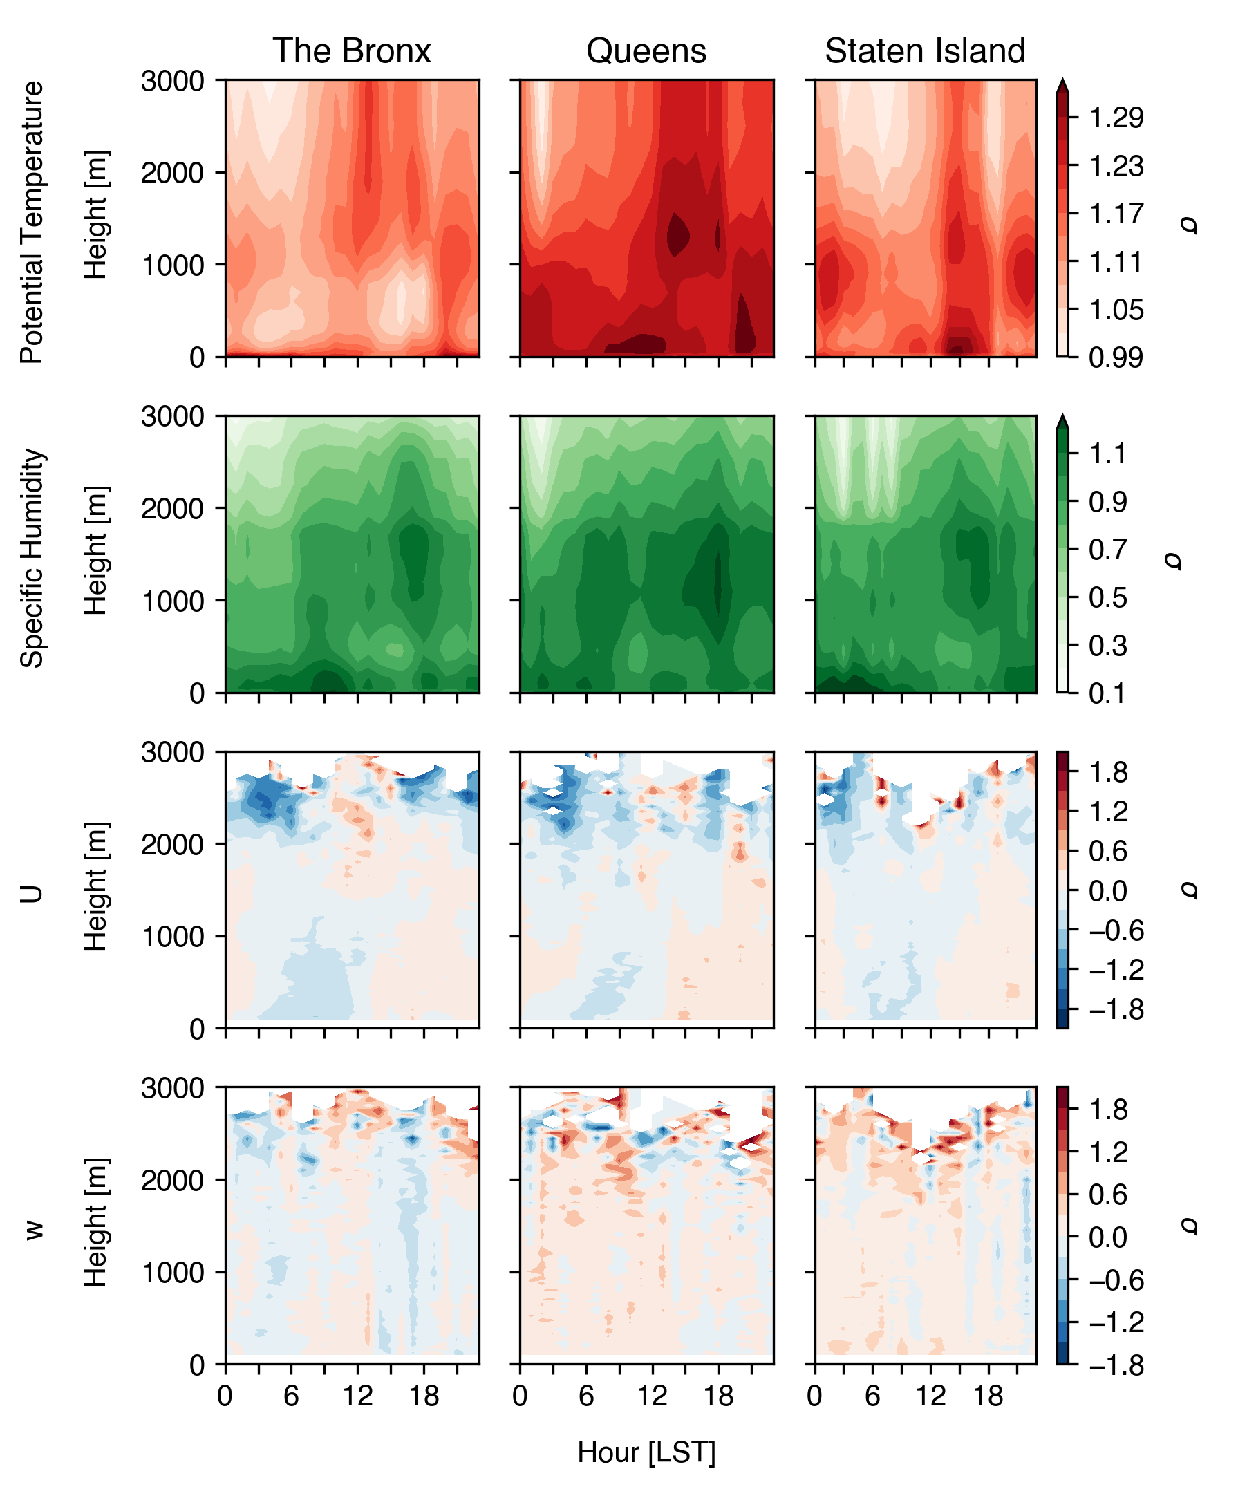
\includegraphics[width=0.75\textwidth]{Figures/heat_wave-normal-anomaly.png}
	\caption{Anomalies during extreme heat events relative to the climatology over the urban boundary layer.}
	\label{fig:extreme-heat-normal-comparison-contours}
\end{figure}

\begin{figure}[ht]
	\centering
	\includegraphics[width=0.75\textwidth]{Figures/heat_wave-normal-profiles-surface}
	\caption{Anomalies of temperature during extreme heat events relative to the climatology at the surface.}
	\label{fig:extreme-heat-normal-comparison-surface}
\end{figure}

\begin{figure}[ht]
	\centering
	\includegraphics[width=0.75\textwidth]{Figures/vertical_profiles-heat_wave-normal-theta.png}
	\caption{Vertical profiles of $\theta$ at the Bronx (a), Queens (b), and Staten Island (c) sites during normal days (blue) and extreme heat events (red).}
	\label{fig:vertical_profiles-heat_wave-normal-theta}
\end{figure}

\FloatBarrier

\subsection{Moisture}
On average, extreme heat events were found to increase the moisture at the surface, as indicated by the diurnal profiles of specific humidity ($q$) (see Figure \ref{fig:extreme-heat-normal-comparison-surface}). This is also consistent across all observed locations in New York City, with mean extreme heat event $q$ exceeding normal $q$ by approximately 1-$\sigma$ over the entire day. Although a distinct diurnal profile exists ($q$ decreases during daytime hours), the diurnal range is smaller in magnitude than temperature. It is also worth noting that the diurnal range is lower for Staten Island than for the Bronx or Queens, suggesting that degree of urbanization has a negative correlation with the diurnal range of $q$, due to sustained low-level moisture from local evapotranspiration from nearby vegetated areas. Similar to surface temperature, the variability of $q$ is significantly lower during heat events (average $ \sigma = \SI{2.14e-03}{\kilo\gram\per\kilo\gram} $) than during normal temperatures (average $ \sigma = \SI{3.18e-03}{\kilo\gram\per\kilo\gram} $). Queens shows exceptional variability in $q$, which may be attributed to the location of the observation site, which is adjacent to Flushing Meadows Corona Park (large open vegetated space), is surrounded by a medium-density urban area on all other sides, and is approximately \SI{4}{\kilo\meter} from Long Island Sound. 

In the boundary layer, the positive $q$ anomalies subside in magnitude between 300 and \SI{600}{\meter}, but increase significantly in the mixed layer, especially during the late morning and early afternoon for all sites. As shown in Figure \ref{fig:extreme-heat-normal-comparison-contours}, the largest anomalies occur between 10:00 and 16:00 LST throughout the mixed layer. With regards to spatial variation in $q$, Staten Island demonstrates a strong positive anomaly overnight through the early morning near the surface, indicating increased low-level moisture transport during extreme heat events, whereas the Bronx and Queens demonstrate a similar phenomenon with a lesser anomaly magnitude. All sites show significant positive $q$ anomalies throughout the day, with the strongest anomaly signal starting in the low-levels throughout the morning and transitioning to the mixed later by mid-afternoon. This trend suggests that the increase in nocturnal low-level moisture corresponds to increased UBL moisture content due to strong vertical mixing throughout the daytime.

This is supported by Figure \ref{fig:vertical_profiles-heat_wave-normal-q}, where vertical profiles of $q$ across all locations show markedly higher $q$ values at the surface during extreme heat events (approximately 1-$\sigma$), with $\frac{dq}{dz}$ values increasing throughout the morning in the mixed layer while low-level $q$ values decrease, indicating vertical transport of moisture and drier low-level conditions during peak insolation. The strong vertical mixing of $q$ can be observed at all sites, where late morning and early afternoon $\frac{dq}{dz}$ values are greater during extreme heat events than normal days. An example can be seen in the Bronx, where $\frac{dq}{dz} > 0$, indicating very efficient vertical moisture transport. 

In addition to environmental contributions to the positive $q$ anomalies during extreme heat events, it is known that anthropogenic contribution of water vapor increases during extreme heat periods. In New York City, most commercial buildings use chilled water coolers for air conditioning. For example, \citet{gutierrez2015} found significant contributions from the air conditioning system to atmospheric water vapor in the lower boundary layer. Similar findings were observed in Beijing \citep{yu2019} and Hong Kong \citep{wang2018}.

\begin{figure}[ht]
	\centering
	\includegraphics[width=0.75\textwidth]{Figures/vertical_profiles-heat_wave-normal-q.png}
	\caption{Vertical profiles of $q$ at the Bronx (a), Queens (b), and Staten Island (c) sites during normal days (blue) and extreme heat events (red).}
	\label{fig:vertical_profiles-heat_wave-normal-q}
\end{figure}

\FloatBarrier

\subsection{UBL dynamics}

\subsubsection{Horizontal winds}
Extreme heat events coincided with a modest reduction of horizontal wind speeds ($U$) in the UBL, as shown in Figure \ref{fig:extreme-heat-normal-comparison-surface}. More specifically, the magnitude of $U$ during extreme heat events is similar in magnitude to $U$ during normal days with the exception of early morning hours and at upper levels of the UBL. As shown in Figure \ref{fig:extreme-heat-normal-comparison-contours}, modest reductions in $U$ ($-1.2 \leq \sigma \leq -0.4$) during extreme heat events are present throughout the UBL from early to mid-morning, with little difference throughout the rest of the day ($-0.4 \leq \sigma \leq 0.4$). Larger deviations between $U$ values are present at the top of the UBL where synoptic conditions become dominant.

Vertical profiles of $U$ for normal and extreme heat events at specific hours provide a more detailed view of the differences in UBL structure. Across all sites, $U$ is similar throughout the UBL during afternoon, evening, and overnight hours. During early morning hours, however, extreme heat event $U$ values decrease by 25 to 50\% throughout the entire UBL (see Figure \ref{fig:vertical_profiles-heat_wave-normal-U}), although both event types present a classical logarithmic wind profile, with surface friction effects present through \SI{500}{\meter}. The reduction in $U$ during extreme heat events is likely due to the presence of an anticyclonic circulation that suppresses the nocturnal low-level jet over New York City \citep{chen1993}. Another phenomenon worth noting is the difference in $U$ profiles above \SI{2000}{\meter}; profiles of $U$ during extreme heat events are more consistent both vertically and spatially (between sites) than during normal days. This phenomenon demonstrates the effect of synoptic meteorological conditions on $U$, as the UBL typically remains below \SI{2500}{\meter}. During extreme heat events, anticyclonic conditions produce more consistent atmospheric conditions relative to normal days, resulting in less variability between heat events than during normal days.

Extreme heat events result in a southwesterly shift in $U$ throughout the UBL. This shift is present most evidently closer to the surface, as shown in Figures \ref{fig:wind_rose-bron}, \ref{fig:wind_rose-quee}, and \ref{fig:wind_rose-stat}, with winds at \SI{100}{\meter} coming primarily from the southwest quadrant. All sites also present secondary maxima with winds approaching from the south and southeast, which suggests effects from the Atlantic sea breeze (effects from the sea breeze will be further discussed in Section \ref{section:sea_breeze_effects}). At \SI{1000}{\meter}, the directionality of prevailing winds becomes more uniform between normal and extreme heat days, as winds primarily approach New York City from the west-southwest. The disparity in wind directions between 100 and \SI{1000}{\meter} suggests that localized wind fields play a more significant role in UBL dynamics at lower levels whereas synoptic-scale atmospheric conditions increasingly dominate with increasing height. Regardless, the uniformity of wind direction during extreme heat relative to normal days indicates that synoptic-scale effects can play a larger role at lower levels due to advection from the continent, especially with regards to thermal advection that leads to the transport of heated inland air masses over New York City \citep{jiang2019, ramamurthy2017b}.

\begin{figure}[ht]
	\centering
	\includegraphics[width=0.75\textwidth]{Figures/vertical_profiles-heat_wave-normal-U.png}
	\caption{Vertical profiles of $U$ at the Bronx (a), Queens (b), and Staten Island (c) sites during normal days (blue) and extreme heat events (red).}
	\label{fig:vertical_profiles-heat_wave-normal-U}
\end{figure}

% Standalone figure option
\begin{figure}[ht]
	\includegraphics[width=0.75\textwidth]{Figures/wind_rose-bron.png}
	\caption{Horizontal winds in the lower-level (100 m) and mid-level of the urban boundary layer over the Bronx.}
	\label{fig:wind_rose-bron}
\end{figure}
\begin{figure}[ht]
	\centering
	\includegraphics[width=0.75\textwidth]{Figures/wind_rose-quee.png}
	\caption{Horizontal winds in the lower-level (100 m) and mid-level of the urban boundary layer over Queens.}
	\label{fig:wind_rose-quee}
\end{figure}
\begin{figure}[ht]
	\centering
	\includegraphics[width=0.75\textwidth]{Figures/wind_rose-stat.png}
	\caption{Horizontal winds in the lower-level (100 m) and mid-level of the urban boundary layer over Staten Island.}
	\label{fig:wind_rose-stat}
\end{figure}

\FloatBarrier

\subsubsection{Vertical motion}
On average, extreme heat events do not appear to produce significant changes in vertical velocity ($w$) relative to normal days. Figure \ref{fig:extreme-heat-normal-comparison-surface} shows average diurnal profiles of $w$ at all locations at \SI{100}{\meter} above ground level, with similar mean values throughout the day between normal days and extreme heat events. During extreme heat events, the variability of $w$ is lesser in the early morning hours and greater in the evening, albeit featuring similar behavior to normal days. This phenomenon is also observed in vertical profiles of $w$ at all locations as shown in Figure \ref{fig:extreme-heat-normal-vertical_profiles-w}. At all locations, overnight and morning profiles of $w$ (0:00 and 6:00 LST) show significantly lower variability in $w$ throughout the UBL with similar magnitudes of mean $w$, although extreme heat days feature low variability in the UBL. Despite similar means and deviations in the early afternoon (12:00 LST), evening profiles (18:00 LST) show significantly higher variability in $w$ below \SI{500}{\meter} than in the mornings at the Queens and Staten Island sites, with the Bronx showing this occurrence extend through the UBL. The similarity in vertical profiles of $w$ may be a result of a balance between large-scale subsidence (due to the presence of high-pressure during extreme heat events) and the effects of increased surface forcings during extreme heat events relative to normal days \citep{dong2018, zhang2009}.

Additionally, updrafts appear to be lesser in magnitude relative to normal days, although upwards vertical motion persists later at all heights within the UBL. This suggests that vertical mixing is more sustained throughout the day during extreme heat events, although thermal plumes seem to be weaker relative to normal days. A case of this in shown at the Bronx site (see Figure \ref{fig:normal-extreme_heat-w-case_study}), where two days - 26 July 2019 (normal) and 29 July 2019 (extreme heat) - are shown with significantly different temporal profiles. On 26 July, the morning UBL is shallow and neutral through 10:00 LST, where mixing begins as evidenced by surface layer variability in $w$, which is followed by a sustained downdraft throughout the mixed layer. At approximately 12:00 LST, a strong plume extends throughout the UBL, initiating significant mixing from the surface throughout the mixed later. This is followed by modest downdrafts throughout the UBL in the afternoon, followed by relatively neutral conditions in the evening and early nighttime hours. In contrast, 29 July demonstrates similar UBL dynamics in the morning hours, followed by modest low-level mixing through the midday hours, with sustained upwards vertical motions through the afternoon and evening over the entire UBL. 

% Vertical quantity comparison timeseries, extreme heat versus normal
\begin{figure}[ht]
	\centering
	\includegraphics[width=0.75\textwidth]{Figures/vertical_profiles-heat_wave-normal-w.png}
	\caption{Vertical profiles of $w$ at the Bronx (a), Queens (b), and Staten Island (c) sites during normal days (blue) and extreme heat events (red).}
	\label{fig:extreme-heat-normal-vertical_profiles-w}
\end{figure}

% Case study of single day vertical velocity, comparison between normal and extreme heat day
\begin{figure}[ht]
	\centering
	\includegraphics[width=0.75\textwidth]{Figures/case_studies/normal-heat_wave-comparison_20190726_20190729-bron.png}
	\caption{Vertical velocity contours at the Bronx site on a normal (26 July 2019) and extreme heat (29 July 2019) day.}
	\label{fig:normal-extreme_heat-w-case_study}
\end{figure}

\FloatBarrier

%%%%% Discuss the observed sea breeze circulation
\section{Effects of the sea breeze circulation} \label{section:sea_breeze_effects} 
Sea breezes in New York City occur as a result of land-sea temperature gradients from two arms of the Atlantic Ocean; the New York Bight to the southeast and Long Island Sound to the northeast. Sea breezes from both bodies increase the complexity of UBL dynamics over New York City due to the coalescence of opposing fronts over the complex urban topography \citep{bornstein1981}. A typical sea breeze event in New York City is defined by calm ambient low-level winds ($\leq$ \SI{5}{\meter\per\second}), the formation of a large land-sea temperature gradient in the mid- to late morning, strong late-morning thermals that promote low-level convergence, and afternoon to early-evening onshore moisture transport and reduction in surface air temperatures (especially in areas closest to the shore) \citep{childs2005, frizzola1963, gedzelman2003}. 

Sea breeze events occurred on approximately 56\% of all days observed. The high frequency of occurrence is  attributable to low-level convergence due to the large land-sea temperature gradient that is common during warmer months \citep{childs2005, gedzelman2003, thompson2007}, as days were chosen exclusively between May and September. Maximum land-sea surface temperature differences during days with identifiable sea breeze events averaged at \SI{12}{\kelvin}, with a strong diurnal profile with the peak difference occurring around midday (see Figure \ref{fig:sea_breeze-lst_sst-diff}). The frequency of occurrence increases when observing days during extreme heat events, as the lack of a strong synoptic wind allows for the sea breeze circulation to become dominant in the metropolitan area \citep{miller2003}. 

% Sea breeze data
\begin{figure}[ht]
	\centering
	\includegraphics[width=0.75\textwidth]{Figures/sea_breeze-lst_sst-diff.png}
	\caption{Temperature difference between Queens and New York Bight.}
	\label{fig:sea_breeze-lst_sst-diff}
\end{figure}

\begin{figure}[ht]
	\centering
	\includegraphics[width=0.75\textwidth]{Figures/sea_breeze-normal-anomaly.png}
	\caption{Anomalies for normal days with a sea breeze relative to normal days without a sea breeze.}
	\label{fig:sea_breeze_normal-normal-anomaly}
\end{figure}

\begin{figure}[ht]
	\centering
	\includegraphics[width=0.75\textwidth]{Figures/sea_breeze_heat_wave-heat_wave_anomaly.png}
	\caption{Anomalies for heat wave days with a sea breeze relative to heat wave days without a sea breeze.}
	\label{fig:sea_breeze_heat_wave_anomaly}
\end{figure}

\FloatBarrier

\subsection{UBL structure during sea breeze events}
During normal days, observations show that the sea breeze reduces temperature and increases moisture content throughout the UBL after 12:00 LST. In Figure \ref{fig:sea_breeze_normal-normal-anomaly}, the standardized anomalies of $\theta$ between normal days with and without a sea breeze are shown, averaged over all days on an hourly basis. Overnight and in the early morning, positive anomalies of $\theta$ are present above the UBL ($\geq$ \SI{1}{\kilo\meter}) until mid-morning, with the Bronx having the most significant anomaly and Staten Island the least. This suggests a decreasing degree of anomalous $\theta$ with decreasing urbanization. This anomaly pattern coincides with a positive $q$ anomaly trend in both the spatiotemporal aspect (peak anomaly occurs above \SI{1}{\kilo\meter} before 8:00 LST) and the magnitude aspect (the Bronx has the most significant early morning anomaly, Staten Island has the least). Later in the day, all sites observe a negative $\theta$ anomaly throughout the UBL despite a negative $q$ anomaly, indicating that sea breeze events during normal days coincide with a cooler and drier daytime UBL before the onset of the sea breeze. Sea breeze effects become apparent during the mid-afternoon with the presence of a significant negative $\theta$ and positive $q$ anomaly in the lower UBL, with Staten Island experiencing effects first (approximately 16:00 LST) and the Bronx experiencing effects last (approximately 19:00 LST). This disparity in times appears to represent the passage of the southeasterly New York Bight, and to a lesser degree, the Long Island Sound sea breeze fronts through New York City, where the onset time correlates with the distance from the bodies of water \citep{bornstein1981}. It is worth noting that the $q$ anomaly is weakest in the Bronx, which suggests that the sea breeze front weakens as it travels inland over New York City.

During extreme heat events, observations show that the sea breeze plays a moderating role on surface conditions by reducing low-level temperatures and increasing low-level moisture content, similar to phenomena observed during normal days. In Figure \ref{fig:sea_breeze_heat_wave_anomaly}, the standardized anomalies of $\theta$ between extreme heat days with and without a sea breeze are shown, averaged over all days. All sites shown that extreme heat days with a sea breeze possess slightly higher values of $\theta$ in the mid-morning, with significant low-level reduction in $\theta$ in the afternoon and evening. On average, the onset of the low-level cooling occurs in Staten Island first at approximately 12:00 LST, with Queens following at approximately 14:00 LST, and the Bronx at about 18:00 LST. It is worth noting that the negative $\theta$ anomalies are stronger in more urbanized areas, as shown by the Bronx and Queens sites. A similar phenomenon is observed by the transport of $q$ as shown in Figure \ref{fig:sea_breeze_heat_wave_anomaly}, with drier conditions throughout the UBL before 12:00 LST and increasing low-level moisture as the day progresses. With regards to onset, $q$ follows a similar pattern to $\theta$ in that the onset time is dependent from distance to the shore. These anomalies present most significantly in the lowest \SI{1000}{\meter} of the UBL after 12:00 LST, which aligns with sea breeze circulation characteristics observed in \citet{frizzola1963}.

\subsection{UBL dynamics during sea breeze events}
Days with identifiable sea breeze events had lower $U$ throughout the majority of the UBL, with the most significant decreases during the nighttime, potentially due to the lessening of onshore flow due to the reduction of the land-sea temperature gradient \citep{pullen2007}, as shown in Figure \ref{fig:sea_breeze-lst_sst-diff}. Vertical motions, however, increased significantly in the Bronx and Queens during the late morning and early afternoon, as shown in Figure \ref{fig:sea_breeze_heat_wave_anomaly}. These anomalies indicate the increased presence of updrafts in urbanized areas which contribute to low-level convergence and the initiation of a localized sea breeze circulation, promoting onshore flow in the afternoon and evening.

During extreme heat days with identified sea breeze circulations, easterly winds increase in frequency in the lower levels of the UBL, as shown in Figure \ref{fig:wind_direction-heat_wave-sea_breeze-histogram}. These winds are the result of onshore flow from the New York Bight (southeasterly) and Long Island Sound (northeasterly). 

During extreme heat days with sea breeze circulations, southeasterly winds increased in frequency compared to all other directions at all locations. The occurrence frequency of southeasterly winds is correlated with the distance between the observation site and the largest body of water in proximity of the metropolitan area (Atlantic Ocean), as Staten Island reported 92.1\% of all winds at \SI{100}{\meter} as southeasterly between 12:00 and 20:00 LST (distance of \SI{6.50}{\kilo\meter} from Lower New York Bay), whereas Queens reported 67.4\% (distance of \SI{16.5}{\kilo\meter}) and Bronx reported 55.6\% (distance of \SI{32.9}{\kilo\meter}) during the same time interval. The disparity in southeasterly winds further demonstrates the spatial extent and progression of the sea breeze front.

For sites near Long Island Sound (the Bronx and Queens), northeasterly winds increased in frequency as well, though not to the same magnitude as southeasterly winds. This disparity in magnitude suggests that the Long Island Sound sea breeze front is weaker than the New York Bight sea breeze front, which aligns with previous studies of sea breeze fronts over New York City \citep{frizzola1963, meir2013}. Northeasterly winds increased in frequency during extreme heat days with sea breeze circulations, with a notable increase in the early morning hours (a likely result of nocturnal low-level motion) and in the evening hours (signal of a Long Island Sound sea breeze). This phenomenon is also apparent in Queens and Staten Island, albeit to a lesser frequency. 

% Histograms cataloguing frequency of wind directions at 100 m between heat wave days without and with a sea breeze.
\begin{figure}[ht]
	\centering
	\includegraphics[width=0.75\textwidth]{Figures/histogram-wind_direction-sea_breeze-100m.png}
	\caption{Occurrence frequency of wind directions during (a) extreme heat days without a detected sea breeze and (b) heat wave days with a detected sea breeze, at \SI{100}{\meter} at all sites.}
	\label{fig:wind_direction-heat_wave-sea_breeze-histogram}
\end{figure}

\FloatBarrier

\section{Discussion and conclusions} \label{section:discussion_conclusion}

% Supporting evidence
Several phenomena observed in this study have been noted in the literature. With regards to heat-related phenomena, the 'heat dome' effect observed through comprehensive multi-city airborne observations in \citet{zhang2020} was observed herein, with a notable increase in temperatures ($\sigma \geq 0.99$) throughout the UBL during extreme heat events. Specifically, the peak temperature anomalies during extreme heat events occurred during the early morning and early afternoon in the surface layer, with secondary maxima in the mixed layer at approximately \SI{1500}{\meter}. The climatology of mixed layer properties provided in this study aligns with findings herein using different observational methods, although on single-city scale, which is beneficial towards understanding the effects of extreme heat within cities and improving our understanding of the relationship between the surface and mixed layers. It is worth noting that this behavior is similar to modeled conditions presented by \citet{ortiz2018} from a series of factor-separation studies using the Weather Research and Forecasting (WRF) model to understand the effects of urbanization on meteorological conditions in New York City. The results showed that surface factors from urban land cover types presented substantial increases to the surface and mixed layer temperatures (6 to \SI{8}{\kelvin} throughout the day). Moreover, simulations showed especially robust early morning (6:00 LST) mixed layer increases in $\theta$ during extreme heat events, which aligns with composite observations shown herein, despite the studies only ranging over a 5-day period for a specific extreme heat event.

With regards to moisture-related phenomena, various studies have shown that there is increased UBL moisture content during extreme heat events \citep{kunkel1996, pyrgou2020, zhang2020}. In particular, the positive anomalies of $q$ are strongest in the surface layer during the morning, which aligns with findings from the Midwestern United States \citep{kunkel1996} and various regions of differing climates \citep{zhang2020}. However, to the authors' knowledge, very few studies have catalogued long-term observations of the vertical structure of moisture in the UBL during extreme heat events. \citet{zhang2020} presented comparisons of the average diurnal vertical structure of $q$ in humid regions (Louisville, Houston, and Philadelphia) and an inland city in a dry inland region (Denver) and showed the differences in the UBL $q$. Louisville and Philadelphia experienced increases in $q$ throughout the UBL, whereas Houston and Denver experienced decreases in low-level $q$, despite Houston being a coastal city in a humid region. This phenomenon was attributed to synoptic-scale moisture transport, where moist air masses from surrounding humid areas paired with local evapotranspiration to increase $q$ in Louisville and Philadelphia, but drier air masses from the Mountain West resulted in lower $q$ values during extreme heat events. The effects of extreme heat on $q$ in New York City resemble those of the cities in humid regions, where humid continental air masses paired with evapotranspiration from vegetated areas surrounding the area to increase $q$ substantially ($0.1 \leq \sigma \leq 1.2$). The influence of localized UBL dynamics (i.e., sea breeze) further increased low-level $q$ as a result of onshore moisture transport, especially during nighttime hours. 

On a larger scale, differences in UBL dynamics have been shown to play a major factor in UBL properties between normal and extreme heat days. As shown herein, a southwesterly shift in winds throughout the UBL coincided with extreme heat events, further highlighting the role of synoptic conditions on the UBL during extreme heat. The increase in temperatures due to this shift in winds has been reported in multiple studies \citep{heaviside2015, jiang2019, ramamurthy2017b}, where the shift in wind direction results in advection of hot air from continental land masses or the advection of heat from nearby urban areas. In the case of New York City, a southwesterly shift in winds places New York City downwind of the continental United States and the north-central New Jersey urban conurbation, both of which may contribute to a hotter UBL during extreme heat events. Moreover, the effect of sea breezes from multiple fronts around New York City creates a complex flow pattern that increases spatial variability in the local meteorology, which has been shown to reduce temperature throughout the UBL \citep{han2022, hirsch2021, lee2021}, albeit contributing to higher moisture content which affects the nocturnal and successive morning UBL structure. 

% Errors and future work
Despite the extensive results provided herein, additional work is required to better improve our understanding of neighborhood-scale spatial qualities of the boundary layer throughout urban areas, especially in those with complex topography and land cover attributes, such as a coastal city. Despite observation sites in 3 of the 5 boroughs, New York City also features a highly variable array of land cover types and features that are not represented in this study. For example, targeting areas in the densest parts of the city (e.g., Midtown Manattan) or furthest from the coast (e.g., central Brooklyn) would be ideal for observing UBL properties in areas of the city most likely to have peak surface temperatures. The variability of building heights throughout New York City, especially in Manhattan, further complicates UBL dynamics and downwind transport \citep{hanna2006, hanna2007}. Moreover, the distance between sites is on the order of the size of a borough, rendering each station unable to be fully representative of neighborhood-scale processes. A potential solution includes a more extensive network of weather and profiling stations (the Oklahoma City Micronet and its usage as described by \citet{basara2010} is a useful example) that allows for more land cover types to be represented.

% Answer the scientific questions posed in the introduction
Based on the observations and their derived quantities, insight was provided into the questions posed in Section \ref{section:introduction};

\begin{enumerate}
	\item Regarding UBL structure, the UBL shows increased temperatures and moisture content throughout its entirety during extreme heat events. Specifically, the surface and lower mixed layer show the most significant increases in temperature and moisture throughout the diurnal cycle. Moreover, the afternoon mixed layer presents a secondary maxima in temperature and moisture increases, suggesting more sustained vertical mixing during extreme heat events. Regarding UBL dynamics, horizontal wind speeds are slightly lower on average during extreme heat events, with the most notable reductions present in the early morning hours and at the UBL height. Additionally, the directionality of horizontal winds becomes predominantly southwesterly and uniform across the UBL during extreme heat events, suggesting increased low-level advection from the continental United States. Differences in vertical motions between normal days and days with extreme heat are not significant when averaged, although extreme heat events were found to correlate with weaker updrafts despite sustaining prolonged positive $w$ values through the evening hours. Extreme heat days were also found to be less variable in terms of UBL structure and dynamics relative to normal days.
	\item Locally, the transport of scalars appears to increase in the vertical direction during extreme heat events in the UBL, although decreased low-level horizontal winds suppresses strong scalar transport zonally and meridionally, especially during morning hours. Despite similar vertical rates of change of scalar quantities between normal days and days with extreme heat, the increase in low-level temperature and moisture content results in significantly higher mixed layer temperature and specific humidity values during extreme heat days. Moreover, extreme heat days appear to promote onshore low-level moisture transport, especially in areas immediately adjacent to the coast. This phenomenon coincides with an increased sea breeze event frequency during extreme heat events. On a larger scale, the vertical uniformity in wind direction throughout the UBL during extreme heat events promotes the advection of scalars southwest of New York City. 
	\item The sea breeze reduces temperatures throughout the UBL after the onset of the sea breeze, which typically occurs in the mid-afternoon in immediate coastal areas and in the evening for areas further inland. The sea breeze also results in nocturnal low-level onshore moisture transport. It is worth noting that during normal days, there was no significant difference in vertical velocities during days with a sea breeze relative to days without a sea breeze, despite a significant reduction in horizontal winds. However, extreme heat days, significantly higher $w$ values occurred through the surface and lower mixed layer during the late morning periods at the Bronx and Queens sites.
	
\end{enumerate}

\section*{Appendix} \label{section:appendix}

\subsection*{Atmospheric pressure}

Atmospheric pressure, $p$, was derived using Equation \ref{eqn:pressure} from observed surface pressure ($p_0$), observed surface temperature ($T_0$), height above the surface ($p$), and the gas constant for dry air ($R$) following the definition provided in \citet{wallace2006}. Note that the virtual temperature correction is neglected in this derivation.

\begin{equation*}\label{eqn:pressure}
	p = p_0 \exp{\frac{-g z}{R T_0}}
\end{equation*}

\subsection*{Potential temperature}

Potential temperature ($\theta$) was derived using Equation \ref{eqn:potential_temperature}, using observed surface temperature ($T_0$), observed surface pressure ($p_0$), height above the surface ($z$), and the gas constant for dry air ($R$), following the definition provided in \citet{wallace2006}.

\begin{equation*}\label{eqn:potential_temperature}
	\theta = T \left(\frac{p_0}{p} \right)^{\frac{R}{c_p}}
\end{equation*}

\subsection*{Specific humidity}

Specific humidity ($q$) was derived using Equation \ref{eqn:specific_humidity} as a function of the mixing ratio ($w$), which in turn is a function of the density of water vapor (also known as \textit{vapor density}) ($\rho_v'$), air temperature ($T$), and the gas constant for water vapor ($R_v$), following the definitions provided in \citet{wallace2006}. 

\begin{equation*}\label{eqn:specific_humidity}
	q = \frac{w}{1+w} = \frac{\frac{\varepsilon \rho_v' R_v T}{p - \rho_v' R_v T}}{1+\frac{\varepsilon \rho_v' R_v T}{p - \rho_v' R_v T}} 
\end{equation*}

% Table displaying symbols used in the 
\captionof{table}{Symbols and abbreviations used in the chapter.}
\label{tab:symbols}
\begin{center}
	\renewcommand{\arraystretch}{1}%
	\begin{tabularx}{0.75\textwidth}{l X}
 		\hline
 		Symbol/Abbreviation & Definition \\
 		\hline
 		$\sigma$ & Standard deviation \\
 		$\theta$ & Potential temperature \\
 		$q$ & Specific humidity \\
 		$U$ & Horizontal wind speed \\
 		$w$ & Vertical velocity \\
 		UBL & Urban boundary layer \\
 		\hline
	\end{tabularx}
\end{center}